\documentclass[UTF8]{ctexart}  % 使用ctexart文档类,适合中文文章
\usepackage{fancyhdr}
\usepackage{pdfpages}

% 使用系统字体
\setCJKmainfont{SimSun} % 宋体
\setCJKsansfont{SimHei} % 黑体
\setCJKmonofont{FangSong} % 仿宋体

% 设置其他字体
\setCJKfamilyfont{kai}{KaiTi} % 楷体
\setCJKfamilyfont{yahei}{Microsoft YaHei} % 微软雅黑
\setCJKfamilyfont{stzhongsong}{STZhongsong} % 华文中宋

\newcommand{\mkai}{\CJKfamily{kai}} % 定义命令切换到楷体
\newcommand{\myahei}{\CJKfamily{yahei}} % 定义命令切换到微软雅黑
\newcommand{\mzhongsong}{\CJKfamily{stzhongsong}} % 定义命令切换到华文中宋

\pagestyle{fancy}
\fancyhf{} % 清除当前设置
\cfoot{\thepage} % 将页码居中显示在页脚
\renewcommand{\headrulewidth}{0pt} % 将页眉横线的宽度设置为零

% \usepackage{fancyhdr}

% \pagestyle{fancy}
% \fancyhf{}
% \fancyhead[C]{\thepage} % 设置 LaTeX 页眉格式

\title{浙江大学校歌}


\begin{document}


\maketitle

\texttt{本节所收录内容,均与浙江大学校歌相关,包括浙江大学校歌歌词、校歌的简谱歌谱、校歌诞生的历史、注释、译文与新解、传唱滋养等
\footnote{文档原电子版由浙江大学上海校友会生仪分会校友谢英杰提供,由江锋整理经\LaTeX 重新编译而成,一切版权归属浙江大学所有。}
\footnote{如文档有误,烦请联系silencejiang@zju.edu.cn进行更正。}
。}

\texttt{浙江大学校歌付诸文言,共有149字,分为三章。首章言说国立大学之精神;次章言说国立浙江大学求是之精神,诠释校训之真谛;末章言说国立浙江大学现今之地位,以及将来之使命。
浙大校歌博大精深,校歌文化深入人心。同时,校歌所阐释的“礼主别异,乐主和同”理念,业已成为浙江大学生动的音乐生活实践的行动指南。}


% {

% 这是宋体(主字体)。

% \textsf{这是黑体(无衬线字体)。}

% \texttt{这是仿宋体(等宽字体)。}

% \mkai 这是楷体。

% \myahei 这是微软雅黑。

% \mzhongsong 这是华文中宋。

% }

\newpage

\begin{flushleft}
    \textsf{\zihao{3}校歌歌词}
\end{flushleft}

\vspace{1em}

\centerline{\textsf{\zihao{-3}浙江大学校歌}}

\vspace{1em}

\centerline{\mkai{词:马一浮 \quad 曲:应尚能}}

\vspace{1em}

\qquad \qquad 大不自多,海纳江河。惟学无际,际于天地。

\qquad \qquad 形上谓道兮,形下谓器。礼主别异兮,乐主和同。

\qquad \qquad 知其不二兮,尔听斯聪。

\vspace{1em}

\qquad \qquad 国有成均,在浙之滨。昔言求是,实启尔求真。

\qquad \qquad 习坎示教,始见经纶。无曰已是,无曰遂真。

\qquad \qquad 靡革匪因,靡故匪新。何以新之,开物前民。

\qquad \qquad 嗟尔髦士,尚其有闻。

\vspace{1em}

\qquad \qquad 念哉典学,思睿观通。有文有质,有农有工。

\qquad \qquad 兼总条贯,知至知终。成章乃达,若金之在熔。

\qquad \qquad 尚亨于野,无吝于宗。树我邦国,天下来同。



\newpage

\begin{flushleft}
    \textsf{\zihao{3}校歌简谱}
\end{flushleft}

{
    \renewcommand{\newpage}{}
    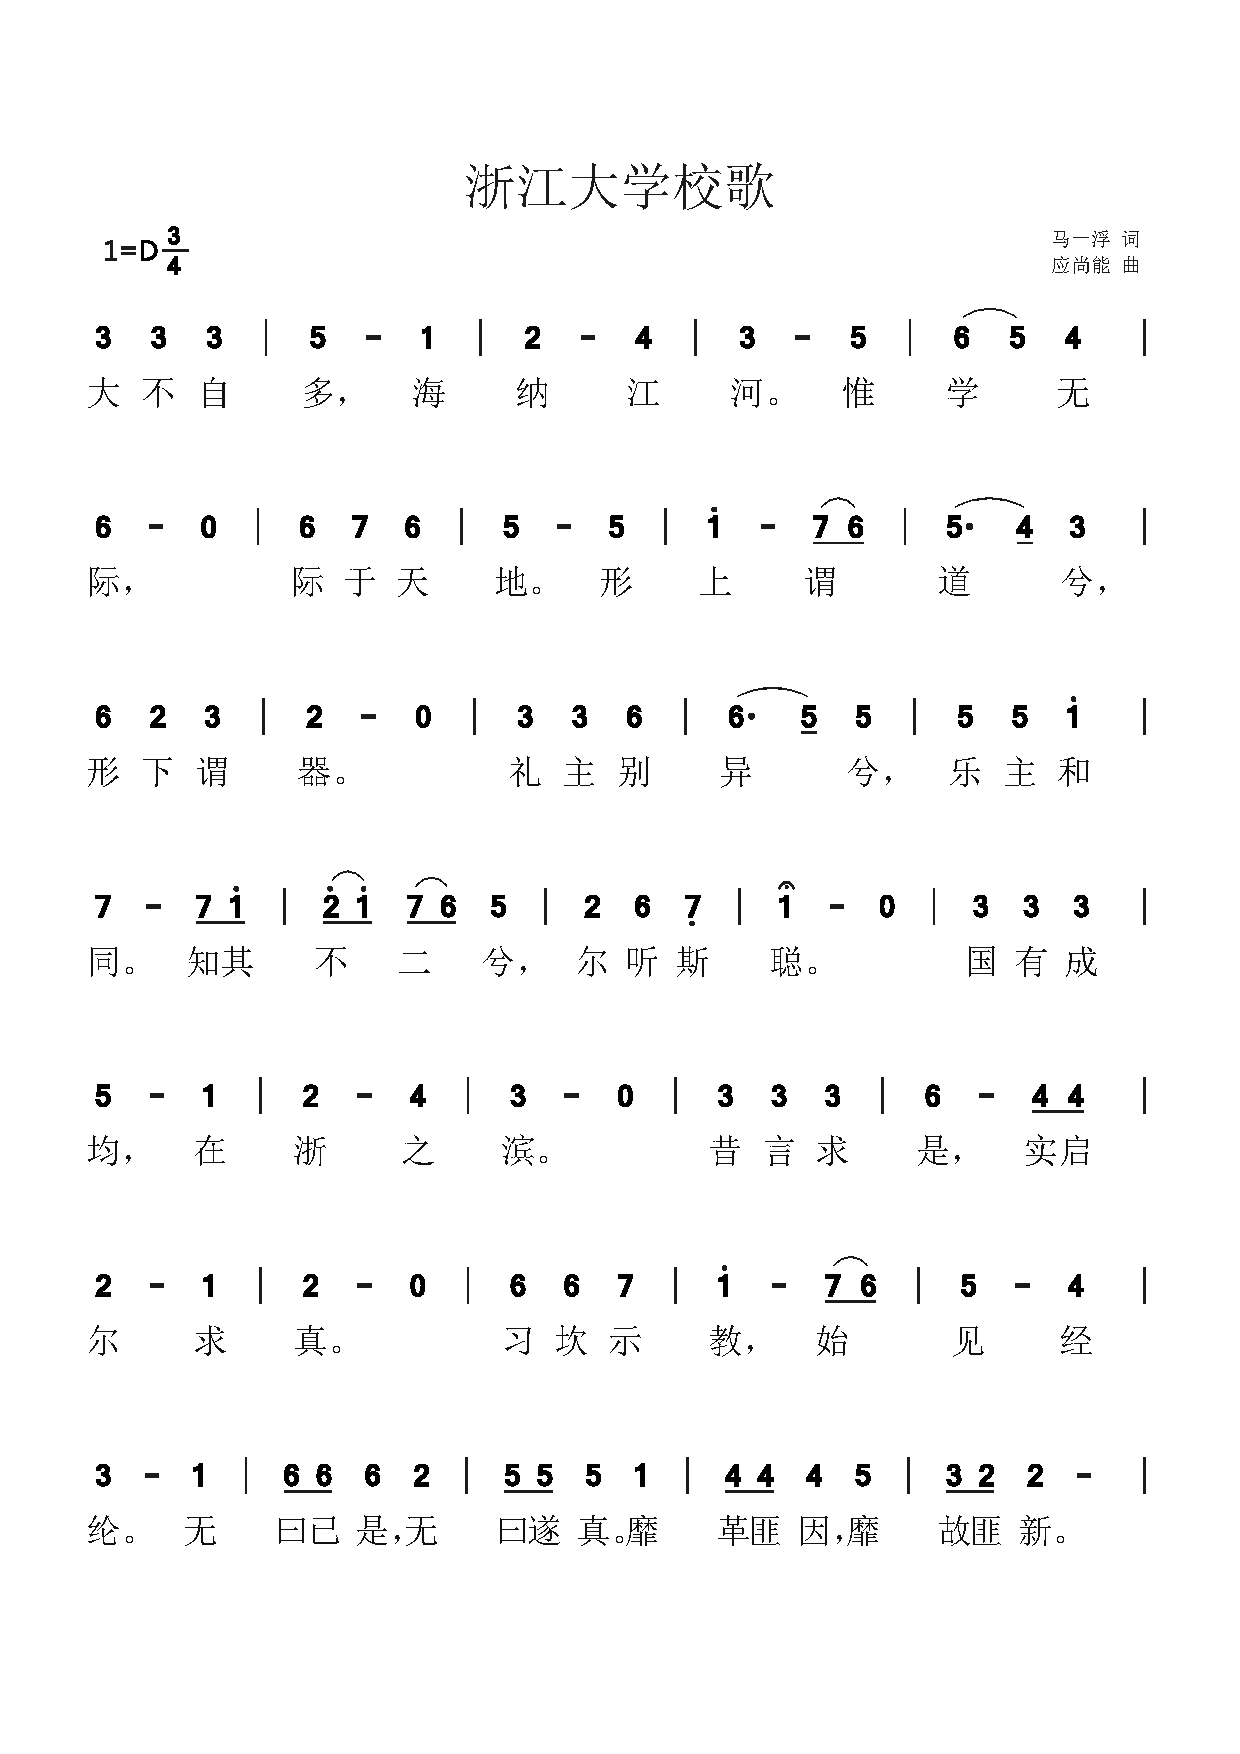
\includepdf[
        pages=1,
        scale=0.8,
        pagecommand={\thispagestyle{fancy}},
        % pagecommand={\pagestyle{fancy}},
        % frame, % remove this line if you don't want outer fram of pdf
    ]{song.pdf}
}

\newpage

{
    \renewcommand{\newpage}{}
    \includepdf[
        pages=2,
        scale=0.8,
        pagecommand={\thispagestyle{fancy}},
        % pagecommand={\pagestyle{fancy}},
        % frame, % remove this line if you don't want outer fram of pdf
    ]{song.pdf}
}

% http://jianpu99.net/
% #============================以下为描述头定义==========================
% V: 1.0
% B: 浙江大学校歌
% Z: 马一浮 词
% Z: 应尚能 曲
% D: D
% P: 3/4
% #============================以下开始简谱主体==========================
% Q: 3 3 3 | 5 - 1 | 2 - 4 | 3 - 5 | (6 5) 4 |
% C: 大不自多, 海纳 江 河。惟学@ 无 
% Q: 6 - 0 | 6 7 6 | 5 - 5 | 1' - (7/ 6/) | (5. 4/) 3 |
% C: 际,@际于天地。形上谓@道@兮,
% Q: 6 2 3 | 2 - 0 | 3 3 6 | (6. 5/) 5 | 5 5 1' |
% C: 形下谓器。@礼主别异@兮,乐主和
% Q: 7 - 7/ 1'/ | (2'/ 1'/) (7/ 6/) 5 | 2 6 7, | 1&yc - 0 | 3 3 3 |
% C: 同。知其不@二@兮,尔听斯聪。@国有成
% Q: 5 - 1 | 2 - 4 | 3 - 0 | 3 3 3 | 6 - 4/ 4/ |
% C: 均,在浙之滨。@昔言求是,实启
% Q: 2 - 1 | 2 - 0 | 6 6 7 | 1' - (7/ 6/) | 5 - 4 |
% C: 尔求真。@习坎示教,始@见经
% Q: 3 - 1 | 6/ 6/ 6 2 | 5/ 5/ 5 1 | 4/ 4/ 4 5 | 3/ 2/ 2 - |
% C: 纶。无曰已是,无曰遂真。 靡革匪因,靡故匪新。
% [fenye]
% Q:  (1 2) 3 | 5 4 3/ 4/ | 5 6 (7/ 1'/) | (2'/ 1'/) (7/ 6/) 5 | 2 6 7, |
% C: 何@以新之,开物前民。嗟@尔@髦@士,尚其有
% Q: 1 - 0 | 3 3 3 | 5 - 1 | 2 - 4 | 3 - 5 |
% C: 闻。@念哉典学,思睿观通。有
% Q: 5 - 5 | 6 - 7 | (1' 7) 6 | 5 - 5 | 1' - (7/ 6/) |
% C: 文有质,有农@有工。兼总条
% Q: 5 - 3 | (6 2) 3 | 2 - 2 | (3. 2/) 3 | 4 - 3 |
% C: 贯,知至@知终。 成章@乃达,若
% Q: 4. 3/ 4 | 5 - 4 | (5. 4/) 5 | 6 - 5 | (6. 5/) 6 |
% C: 金之在熔。尚亨@于野,无吝@于
% Q: 7 - 0 | (2'/ 1'/) (7/ 6/) (5/ 4/) | 3 - 0 | 2 6&yc 7, 1&yc - 0 ||
% C: 宗。@树@我@邦@国,@天下来同。


\newpage

\begin{flushleft}
    \textsf{\zihao{3}校歌历史}
\end{flushleft}


1938年11月19日,在广西宜山,竺可校长主持校务会议,会议决定以“求是”为浙江大学校训,并决定请著名国学家马一浮写校歌歌词。
马一浮作的这首歌词,因为引用了较多的古典,用的是文言文,不太通俗,且读起来有时比较拗口,竺校长曾考虑改写,但他又觉得,马老作的歌词虽文理艰深,
但含义深远,很能体现浙江大学所追求的求是精神,因此,这首“大不自多”歌仍请著名作曲家、当时的国立中央音乐学院的应尚能教授谱曲,并经校务会议通过,
正式定为浙江大学校歌。

\vspace{2em}

\begin{flushleft}
    \textsf{\zihao{3}校歌注释}
\end{flushleft}

{
\mkai{马一浮先生在创作完成《浙江大学校歌》歌词后,曾撰写了《拟浙江大学校歌附说明》一文,以“略为注释”。该文被刘梦溪主编、河北教育出版社
1996年8月出版的《中国现代学术经典·马一浮卷》收录(见该书第84-87页),现作为解读《浙江大学校歌》文义的重点推荐材料全文转引如下。}

\vspace{1em}

\texttt{大不自多,海纳江河。惟学无际,际于天地。形上谓道兮,形下谓器。礼主别异兮,乐主和同。知其不二兮,尔听斯聪。}

\texttt{国有成均,在浙之滨。昔言求是,实启尔求真。习坎示教,始见经纶。无曰已是,无曰遂真。靡革匪因,靡故匪新。何以新之,开物前民。嗟尔髦士,尚其有闻。}

\texttt{念哉典学,思睿观通。有文有质,有农有工。兼总条贯,知至知终。成章乃达,若金之在容\footnote{此处原电子稿即为“金之在容”,下句的“尚无于野”亦如此。}。
尚无于野,无吝于宗。树我邦国,天下来同。}

\vspace{1em}
}

案今国立大学,比于古之辟雍。古者飨射之礼于辟雍行之,因有燕乐歌辞,燕飨之礼,所以仁宾客也。故歌《鹿鸣》以相宴乐,歌《四牡》《皇皇者华》以相劳苦,厚之至也。
食三老五更于太学,必先释奠于先师,今皆无之。学校歌诗唯用于开学毕业,或因特故开会时,其义不同于古。所用歌辞,乃当述立教之意,师弟子相勖勉诰诫之言,
义与箴诗为近。辞不厌朴,但取雅正,寓教思无穷之旨,庶几歌者听者咸可感发兴起,方不失乐教之义。《学记》曰:“大学始教,皮弁祭菜,示敬道也。
宵雅肄三,官其始也。”此见古者礼乐之教,浃于人心,然后政成民和,国家以安。明堂为政之所从出,辟雍为教之所由兴,其形于燕飨歌辞者,笃厚深至如此,
犹可见政教相通之义,此治化之本也。《论语》曰:“诵诗三百,授之以政不达,虽多亦奚以为。”今作乐安歌宜知此意。

今所拟首章,明教化之本。体用一原,显微无间。道器兼该,礼乐并得。以救时人歧而二之之失。言约义丰,移风易俗之枢机,实系于此。

次章,出本校缘起。以求是书院为前身,闻已取求是二字为校训。今人人皆知科学所以求真理,其实先儒所谓事物当然之则,即是真理。
事物是现象,真理即本体。理散在万事万物,无乎不寓。所谓是者,是指分殊。所谓真者,即理一也。凡物有个是当处,乃是天地自然之序,物物皆是当。
交相为用,不相陵夺即是天地自然之和。是当,犹今俗言停停当当,亦云正当。序是礼之本,和是乐之本,此真理也。六经无真字,老庄之书始有之。
《易》多言贞,贞者正也。以事言,则谓之正义。以理言,则谓之真理。或曰诚。或曰无妄。皆真义也。是字从正,亦贞义也。以西洋哲学真善美三义言之,
礼是善,乐是美,兼善与美斯真矣。《易》曰:“天下之动贞夫一者也。”《华严》谓之一真法界,与《易》同旨。故谓求是乃为求真之启示,
当于理之谓是,理即是真,无别有真。《易》曰:“水洊至,习坎,君子以常德行。”习教事,义谓水之洊至,自涓流而汇为江海,顺其就下之性而无骤也。
君子观于此象,而习行教化之事,必其德行恒常,然后人从之。本校由求是蜕化而来,今方渐具规模,初见经纶之始,期其展也大式,如水之洊至,
故用习坎之义。取义于水,亦以其在浙也。无曰四句,是诫勉之词。明义理无穷,不可自足。勿矜创获,勿忘古训,乃可日新。
开物成务,前民利用,皆先圣之遗言,今日之当务。前民之前,即领导之意。傅说之告高宗曰:“学于古训乃有获。”今日学子尊今而蔑古,蔽于革而不知因,此其失也。
温故知新可以为师,教者所以长善而救其失,此章之言,丁宁谆至,所望于浙大者深矣。末章之意,与首章相应。首言体之大,末言用之弘。
念终始典于学是说命文,典者常也。久于其道而天下化成,乃终始典学之效。成山假就于始篑,修涂托至于初步,要终者必反始,始终如一也。
思曰睿,睿作圣。是《洪范》文。观其曾通以行其典礼,是《易·系辞》文。知至至之可与几也,知终终之可与存义也,《易·乾·文言》文。
知至即始条理事,知终即终条理事,“同人于野,亨”,《易·同人》卦辞。“同人于宗,吝”,《同人》六二爻辞。野者旷远之地,惟廓然大公,斯放之皆准,而无睽异之情,故亨。
宗者族党之称,谓私系不忘,则畛域自封,终陷褊狭之过,故吝。学术之有门户,政事之有党争,国际之有侵伐,爱恶相攻,喜怒为用,皆是同人于宗致吝之道。
学也者所以通天下之志,故教学之道,须令心量广大,绝诸偏曲之见,将来造就人才,见诸事业,气象必迥乎不同,方可致亨。又今学校方在播迁之中,远离乡土,亦有同人于野之象。
大学既为国立,应无地方限制。若谓必当在浙,亦是同人于宗,吝道也。然此之寓意甚小,无关宏旨。他日平定后还浙,长用此歌,于义无失。
又抗战乃一时事变,恢复为理所固然。学校不摄兵戎,乐章当垂久远。时人或以勾践沼吴为美谈,形之歌咏,以寓复兴之志,亦是引喻失义。
若淮夷率服,在泮献功,自系当来之事,故抗战情绪不宜羼人。歌辞文章自有体制,但求是当,无取随人。歌辞中用语多出于经,初学不曾读经者,或不知来历,即不明其意义。
又谱入曲调,所安声律,亦须与词中意旨相应,故欲制谱之师,于此歌辞深瞭解,方可期于尽善。因不避迂妄,略为注释,如其未当,以俟知者。


\vspace{2em}

\begin{flushleft}
    \textsf{\zihao{3}校歌译文}
\end{flushleft}

{
\mkai{1992年4月浙江大学95周年校庆期间,曾任宁波大学校长的浙江大学土木系44届毕业生朱兆祥(前浙大合唱团团长)和浙江大学外文系46届毕业生邓爽,
应浙大合唱团老团员的建议,把校歌歌词逐句对应式地译成了白话文,后来又在征询有关专家意见后,稍加修改,形成译文,以便阅读。}
}

\vspace{2em}

大海浩瀚而不自满,所以能容纳千万条江河。

学问的世界无边无际,抵达天地的尽头。

形而上的称为道,形而下的称为器。

礼制主导世界的差异,音乐使社会和谐共存。

明白其中的辩证统一关系,就会更加聪慧明智。

\vspace{2em}

有一所国立大学,在中国东南的浙水之滨。

它以求是为宗旨,其实就是启迪人们求真。

持之以恒潜心教学,才能逐步加深对世界的认识。

不要说已把握事物本质,也不要说已穷尽真理。

没有什么变革不需要继承,没有什么传统不可以创新。

怎样改革创新?实践探索奋勇争先。

诸位年轻的英才,应当明了这些重要道理。

\vspace{2em}

要致力于学问,以达到思想睿智、见识通达,

我们有人文、科学、农业、技术多种学科。

要融会贯通,掌握知识的源流和实践运用。

像金子在熔炉中一样,锻造伟大的成果。

立足民众才能取得真正的成功,不要被宗派门户所束缚。

努力振兴祖国,使世界各国人民和谐共处。

\vspace{2em}

\begin{flushleft}
    \textsf{\zihao{3}校歌新解}
\end{flushleft}

大——永不自满,像大海包容江河,

学——辽阔无际,广胸怀察天观地。

天地间形而上者称道,形而下者为器,

人类社会则有制度统摄差异,艺术促进和谐。

明白它们是统一的客体,学问才有洞察之力。

\vspace{2em}

有一所中国最好的大学,在浙水之滨,

她曾经以求是为名,实质是启迪大学求真。

真理需要恒久地探索习教,才能一窥经纶,

所以莫言已达事物真谛,更莫言已穷尽真理。

没有什么革新不需要继承,没有什么旧例不可以创新,

如何改革创新?唯有走在民众前列勇于探求实践。

诸位青年才俊,要认识这样的科学路径。

\vspace{2em}

专注于学问,才能思想深刻,识解通明。

我们有人文、科学、农业、技术多种学科,

要善于分析综合,掌握知识的源流走向。

真金在熔炉中才会闪现,伟大的成果在锤炼中产生,

绝不能固守宗派门户,走入人民大众才会找到通达之路,

大家努力振兴祖国,使世界各国心驰神往和平共处。

\newpage

\begin{flushleft}
    \textsf{\zihao{3}传唱滋养}
\end{flushleft}


传唱校歌是浙江大学师生自觉的文化行动。从2001年开始,浙江大学的本科新生一进校园就要在学长组的带领下学唱校歌,并开展校歌大合唱比赛。
2006年10月,学校组织开展“唱响浙大”活动,教职员工以及所有校院两级领导均加入相应的合唱队伍参与校歌演唱比赛。不久之后,全校师生大都能唱校歌。
在每次重大的典礼仪式上,台上台下师生合唱校歌成了一种不可或缺的传承。学校还把全校固定办公电话铃声换成校歌音乐彩铃,意在感染更多的人。

校歌经代代传唱,其内涵已深入人心,成为海内外浙大人的共同心声,是学校的文化瑰宝。2015年11月27日,学校公布了“求是创新”校训,“勤学、修德、明辨、笃实”的共同价值观,
“海纳江河、启真厚德、开物前民、树我邦国”的浙大精神这一最新系统表述。校党委书记金德水说:“对照校歌歌词大家能够发现,浙大精神表述语出校歌,
是结合校歌内涵及当代大学使命提炼而成的。可以说,浙大校歌是我们实现中国特色世界一流大学宏伟办学梦想的精神食粮,充分体现了文以贯道的要求。”

浙大校歌文蕴深厚,曲韵典雅,含义深邃,在教育部新闻办公室官方微博2014年发起的“最受欢迎的高校校歌”评选中,荣登高校“十大校歌”排名榜首,被誉为“最美校歌”。
校长吴朝晖指出,浙大校歌集中体现了浙江大学的办学理念和大学精神,凝聚着所有浙大人求是创新的不懈追求,校歌及其诠释的“海纳江河、启真厚德、开物前民、树我邦国”的浙大精神,
为浙江大学的改革发展和文化传承提供了源源不断的强大精神动力。


\end{document}
